\newcommand{\sref}[1]{SLIDE \ref{#1}}

\newcommand{\mypage}[2]{%
\begin{center}%
{\begin{minipage}[t]{3.8in}{#1}\end{minipage}}%
{\begin{minipage}[t]{3.8in}{#2}\end{minipage}}%
\end{center} }

\newcommand{\mypageA}[2]{%
\begin{center}%
{\begin{minipage}[t]{4.0in}{#1}\end{minipage}}%
{\begin{minipage}[t]{3.6in}{#2}\end{minipage}}%
\end{center} }

\newcommand{\mypageB}[2]{%
\begin{center}%
{\begin{minipage}[t]{5.1in}{#1}\end{minipage}}%
{\begin{minipage}[t]{2.5in}{#2}\end{minipage}}%
\end{center} }

\newcommand{\mypageC}[2]{%
\begin{center}%
{\begin{minipage}[t]{3.8in}{#1}\end{minipage}}%
{\begin{minipage}[t]{3.8in}{#2}\end{minipage}}%
\end{center} }

\newcommand{\threepage}[3]{%
\begin{center}%
{\begin{minipage}[t]{2.55in}{#1}\end{minipage}}%
{\begin{minipage}[t]{2.55in}{#2}\end{minipage}}%
{\begin{minipage}[t]{2.55in}{#3}\end{minipage}}%
\end{center} }

\newcommand{\rightLarrow} 
{\mbox{
	\begin{picture}(0,10)(0,0)
	\put(0,15){\line(0,-1){10}}
	\put(1,5){\oval(2,2)[bl]}
%	\put(2,5){\vector(1,0){16}}
%	\put(2,3){\line(1,0){11}}
%	\put(18,5){\line(-1,-1){3}}
%	\put(18,5){\line(-1,1){10}}
	\end{picture}
\hspace*{-0.115in}
{\large $\rightarrow$}
}}

% Define some standard colors
\newrgbcolor{ltgreen}{0.4 0.9 0.4}
\newrgbcolor{dkgreen}{0.0 0.50 0.0}
\newrgbcolor{ltblue}{0.4 0.4 0.9}
\newrgbcolor{dkblue}{0.0 0.0 0.45}
\newrgbcolor{ltred}{0.9 0.4 0.4}
\newrgbcolor{dkred}{0.45 0.0 0.0}
\newrgbcolor{red}  {1.0 0.0 0.0}
\newrgbcolor{maroon}{0.45 0.0 0.0}
%\newrgbcolor{maroon}{0.5 0.0 0.2}
\newrgbcolor{medbrown}{0.5 0.3 0.1}
\newrgbcolor{ltpurple}{0.8 0.0 0.8}
\newrgbcolor{dkpurple}{0.2 0.0 0.2}

% Define a title page layout
\newcommand{\tpage}[6]%
{\center
         {\red\shadowbox{\parbox[b]{#1}{\center\Huge\bf\sc{#2}}}} \\
                       \vspace*{1in}
                       \center{\LARGE \bf \sc \dkblue {#3}}             \\
                       \vspace*{0.1in}
                       \center{\LARGE \bf \sc \dkblue {#4}}             \\
                       \vspace*{0.1in}
                       \center{\LARGE \bf \sc \dkblue {#5}}             \\
                       \vspace*{0.2in}
                       \center{\LARGE \bf \sc \dkblue {#6}}             }

% Define a standard header
\newcommand{\heading}[1]{\vspace*{-0.1in}\center {\dkgreen \shadowbox{\bf \sc {#1}}}}
%\newcommand{\heading}[1]{ {\vspace*{-0.1in} \dkgreen \shadowbox{\center \bf \sc {#1}}}}
%\newcommand{\heading}[1] {\dkgreen\shadowbox{\center\LARGE\bf\sc{#1}}}
%\newcommand{\heading}[1] {\dkgreen\shadowbox{#1}}

% Set the symbols for the item hierarchy
\renewcommand{\labelitemi}{\mbox{$\bullet$}}
\renewcommand{\labelitemii}{\mbox{$\circ$}}
\renewcommand{\labelitemiii}{\mbox{$\diamond$}}
\renewcommand{\labelitemiv}{\mbox{$\triangleright$}}

% Set colors and sizes for item entries
% new versions
\newcommand{\itemn}    [1]{ \normalsize \item \dkblue   {#1}}
\newcommand{\itemnGR}  [1]{ \normalsize \item \dkgreen  {#1}}
\newcommand{\itemnRD}  [1]{ \normalsize \item \red      {#1}}
\newcommand{\itemlGR}  [1]{ \large      \item \dkgreen  {#1}}
\newcommand{\iteml}    [1]{ \large      \item \dkblue   {#1}}
\newcommand{\itemlRD}  [1]{ \large      \item \red      {#1}}
\newcommand{\itemL}    [1]{ \Large      \item \dkblue   {#1}}
\newcommand{\itemLGR}  [1]{ \Large      \item \dkgreen  {#1}}
\newcommand{\itemLRD}  [1]{ \Large      \item \red      {#1}}
\newcommand{\itemLA}   [1]{ \LARGE      \item \dkblue   {#1}}
\newcommand{\itemLAGR} [1]{ \LARGE      \item \dkgreen  {#1}}
\newcommand{\itemii}   [1]{ \large      \item \dkpurple {#1}}
\newcommand{\itemiia}  [1]{ \normalsize \item \dkpurple {#1}}
\newcommand{\itemiii}  [1]{ \normalsize \item \dkgreen  {#1}}
\newcommand{\itemiv}   [1]{ \normalsize \item \medbrown {#1}}

% Old versions
% \newcommand{\itemn}    [1]{\item \dkblue    \normalsize   {#1}}
% \newcommand{\itemnGR}  [1]{\item \dkgreen   \normalsize   {#1}}
% \newcommand{\itemnRD}  [1]{\item \dkred     \normalsize   {#1}}
% \newcommand{\itemlGR}  [1]{\item \dkgreen   \large        {#1}}
% \newcommand{\iteml}    [1]{\item \dkblue    \large        {#1}}
% \newcommand{\itemlRD}  [1]{\item \dkred     \large        {#1}}
% \newcommand{\itemL}    [1]{\item \dkblue    \Large        {#1}}
% \newcommand{\itemLGR}  [1]{\item \dkgreen   \Large        {#1}}
% \newcommand{\itemLRD}  [1]{\item \dkred     \Large        {#1}}
% \newcommand{\itemLA}   [1]{\item \dkblue    \LARGE        {#1}}
% \newcommand{\itemLAGR} [1]{\item \dkgreen   \LARGE        {#1}}
% \newcommand{\itemii}   [1]{\item \dkpurple  \large        {#1}}
% \newcommand{\itemiia}  [1]{\item \dkpurple  \normalsize   {#1}}
% \newcommand{\itemiii}  [1]{\item \dkgreen   \normalsize   {#1}}
% \newcommand{\itemiv}   [1]{\item \medbrown  \normalsize   {#1}}

\newcommand{\nobiteml}    [1] {\item[] \dkblue    \large      {#1}}
\newcommand{\nobitemlGR}  [1] {\item[] \dkgreen   \large      {#1}}
\newcommand{\nobitemL}    [1] {\item[] \dkblue    \Large      {#1}}
\newcommand{\nobitemLGR}  [1] {\item[] \dkgreen   \Large      {#1}}
\newcommand{\nobitemLA}   [1] {\item[] \dkblue    \LARGE      {#1}}
\newcommand{\nobitemLAGR} [1] {\item[] \dkgreen   \LARGE      {#1}}
\newcommand{\nobitemii}   [1] {\item[] \dkpurple  \large      {#1}}
\newcommand{\nobitemiia}  [1] {\item[] \dkpurple  \normalsize {#1}}
\newcommand{\nobitemiii}  [1] {\item[] \dkgreen   \normalsize {#1}}
\newcommand{\nobitemiv}   [1] {\item[] \medbrown  \normalsize {#1}}

% Define a custom Slideframe Style
\newslideframe{Logo}%
{\boxput(-0.95,0.92){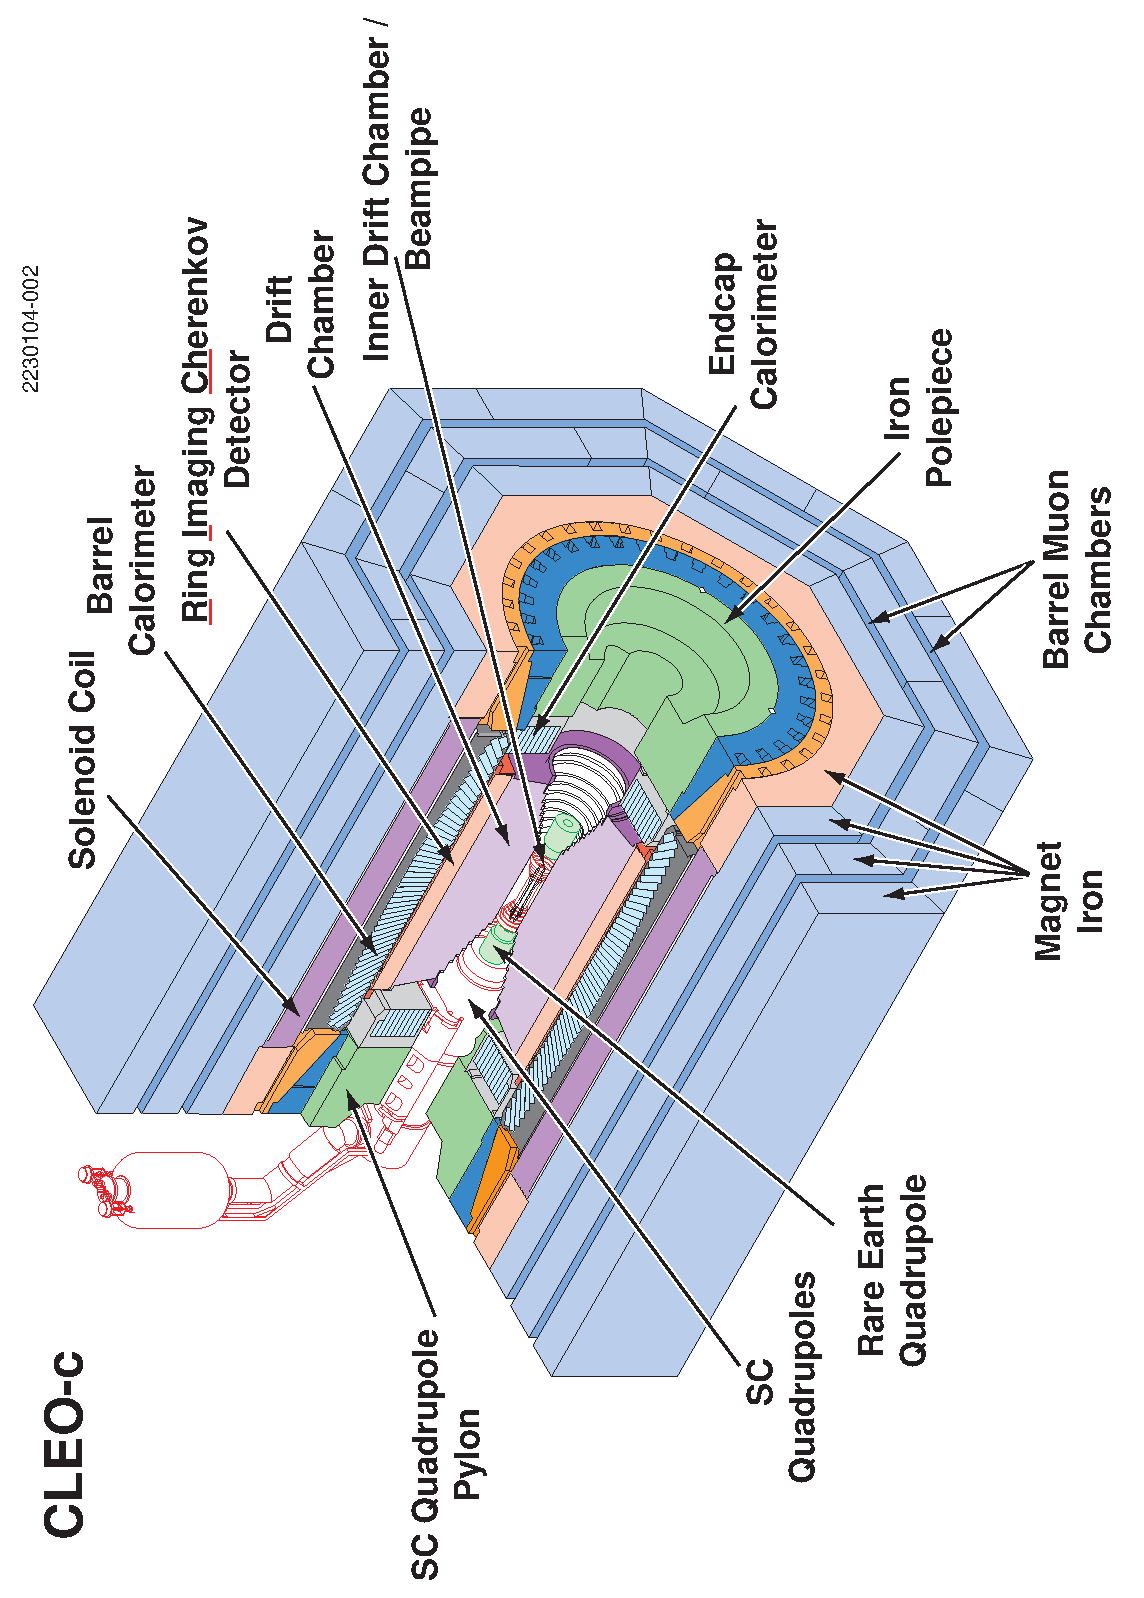
\psfig{file=/home/palmer/tex/cleo/cleo.eps,height=1.0in} \hskip -0.52in {\dkblue \large \it \raisebox{0.92in}[1.0in][-0.1in]{CLEO}} }{#1}}

% Define a custom Page Style
%\newpagestyle{conference}%
%  {\dkblue \conftitle  \hfil \talktitle \hfil \hskip 1.4in \talkdate}
%  {\dkblue \myname \hfil \affil \hfil \hskip 1.0in \thepage}

\newpagestyle{conference}%
  {\dkblue              \hfil                               \thepage}
  {\dkblue \myname      \hfil \talktitle \hfil              \talkdate}

\newpagestyle{conf_nopage}%
  {\dkblue              \hfil                               }
  {\dkblue \myname      \hfil \talktitle \hfil              \talkdate}

\newcommand{\ra}       {\mbox{$\rightarrow$}}


% Incorporate some standard commands and decays
% Lots of this comes from Jim Alexander's definitions

\newcommand{\xxx}	{\mbox{$xxx$}}
\newcommand{\mev}	{\mbox{${\rm MeV}$~}}
\newcommand{\gev}	{\mbox{${\rm GeV}$~}}
\newcommand{\micron}	{\mbox{$\mu{\rm m}$}}
\newcommand{\about}	{\mbox{$\sim$}}
\newcommand{\implies}	{\mbox{${\Longrightarrow}$}}
\newcommand{\stat}	{\mbox{$_{\rm stat}$}}
\newcommand{\syst}	{\mbox{$_{\rm syst}$}}

\newcommand{\LambdaPpi} {\mbox{$\Lambda \rightarrow p \pi^-$~}}
\newcommand{\BDstar}    {\mbox{$\bar{B^0} \rightarrow D^{*+} l^- 
								\bar{\nu}$\ }}
\newcommand{\BBbar}     {\mbox{${B\bar{B}}$\ }}
\newcommand{\DDbar}     {\mbox{${D\bar{D}}$\ }}
\newcommand{\upsone}    {\mbox{${\Upsilon (1s)}$\ }}
\newcommand{\upstwo}    {\mbox{${\Upsilon (2s)}$\ }}
\newcommand{\upsthree}  {\mbox{${\Upsilon (3s)}$\ }}
\newcommand{\upsfour}   {\mbox{${\Upsilon (4s)}$\ }}
\newcommand{\etapr}	{\mbox{${\eta^\prime}$}}
\newcommand{\bsg}	{\mbox{$b\to s\gamma$}}
\newcommand{\bsll}	{\mbox{$b\to s\ell^+\ell^-$}}
\newcommand{\xs}	{\mbox{${X_s}$}}
\newcommand{\egam}	{\mbox{$E_\gamma$}}
%\newcommand{\bbbar}     {\mbox{$B\bar B$}}
\newcommand{\qqb}	{\mbox{$q\bar q$}}
\newcommand{\ee}	{\mbox{$e^+e^-$}}
\newcommand{\hh}	{\mbox{$h^+h^-$}}
\newcommand{\eeqq}	{\mbox{$ee\to\qqb$}}
\newcommand{\mm}	{\mbox{$\mu^+\mu^-$}}
\newcommand{\emu}	{\mbox{$e^+\mu^-$}}
\newcommand{\see}	{\mbox{$s e^+e^-$}}
\newcommand{\smm}	{\mbox{$s \mu^+\mu^-$}}
\newcommand{\sem}	{\mbox{$s e^+\mu^-$}}
\newcommand{\llb}	{\mbox{$\ell\bar\ell$}}
\newcommand{\branch}    {\mbox{${\cal B}$}}
\newcommand{\amp}    	{\mbox{${\cal A}$}}
\newcommand{\lum}    	{\mbox{${\cal L}$}}
\newcommand{\like}    	{\mbox{${\cal L}$}}
\newcommand{\fisher}    {\mbox{${\cal F}$}}
\newcommand{\taunu}	{\mbox{$\tau\bar\nu_\tau$}}
\newcommand{\munu}	{\mbox{$\mu\bar\nu_\mu$}}
\newcommand{\enu}	{\mbox{$e\bar\nu_e$}}
\newcommand{\pvec}	{\mbox{$\vec{p}$}}
\newcommand{\ebeam}	{\mbox{$E_{\rm beam}$}}
\newcommand{\hpm}	{\mbox{$h^\pm$}}
\newcommand{\costhr}	{\mbox{$\cos \theta_{\rm thr}$}}
\newcommand{\Kpi}	{\mbox{$K\pi$}}
\newcommand{\Pipi}	{\mbox{$\pi\pi$}}
\newcommand{\KK}        {\mbox{$KK$}}
\newcommand{\bdkbig}	{\mbox{$B^+\to \bar D^0 K^+$}}
\newcommand{\bdklittle}	{\mbox{$B^+\to D^0 K^+$}}
\newcommand{\dzero}	{\mbox{${D^0}$}}
\newcommand{\dzerobar}	{\mbox{$\overline {D^0}$}}

\newcommand{\jimexp}[1]	{\mbox{${\rm e}^{{#1}}$}}

\newcommand{\vud}	{\mbox{$V_{ud}$}}
\newcommand{\vcd}	{\mbox{$V_{cd}$}}
\newcommand{\vtd}	{\mbox{$V_{td}$}}
\newcommand{\vus}	{\mbox{$V_{us}$}}
\newcommand{\vcs}	{\mbox{$V_{cs}$}}
\newcommand{\vts}	{\mbox{$V_{ts}$}}
\newcommand{\vub}	{\mbox{$V_{ub}$}}
\newcommand{\vcb}	{\mbox{$V_{cb}$}}
\newcommand{\vtb}	{\mbox{$V_{tb}$}}

\newcommand{\avub}	{\mbox{$|V_{ub}|$}}
\newcommand{\avtd}	{\mbox{$|V_{td}|$}}
\newcommand{\avts}	{\mbox{$|V_{ts}|$}}
\newcommand{\avus}	{\mbox{$|V_{us}|$}}
\newcommand{\avcb}	{\mbox{$|V_{cb}|$}}
\newcommand{\avtb}	{\mbox{$|V_{tb}|$}}
\newcommand{\avud}	{\mbox{$|V_{ud}|$}}

\newcommand{\de}	{\mbox{$\Delta E$}}
\newcommand{\mb}	{\mbox{$M_B$}}

\newcommand{\emone}	{\mbox{${10^{-1}}$}}
\newcommand{\emtwo}	{\mbox{${10^{-2}}$}}
\newcommand{\emthree}	{\mbox{${10^{-3}}$}}
\newcommand{\emfour}	{\mbox{${10^{-4}}$}}
\newcommand{\emfive}	{\mbox{${10^{-5}}$}}
\newcommand{\emsix}	{\mbox{${10^{-6}}$}}
\newcommand{\emseven}	{\mbox{${10^{-7}}$}}
\newcommand{\emeight}	{\mbox{${10^{-8}}$}}
\newcommand{\emnine}	{\mbox{${10^{-9}}$}}
\newcommand{\emten}	{\mbox{${10^{-10}}$}}
\newcommand{\emeleven}	{\mbox{${10^{-11}}$}}
\newcommand{\emtwelve}	{\mbox{${10^{-12}}$}}
\newcommand{\epone}	{\mbox{${10^{1}}$}}
\newcommand{\eptwo}	{\mbox{${10^{2}}$}}
\newcommand{\epthree}	{\mbox{${10^{3}}$}}
\newcommand{\epfour}	{\mbox{${10^{4}}$}}
\newcommand{\epfive}	{\mbox{${10^{5}}$}}
\newcommand{\epsix}	{\mbox{${10^{6}}$}}
\newcommand{\epseven}	{\mbox{${10^{7}}$}}
\newcommand{\epeight}	{\mbox{${10^{8}}$}}
\newcommand{\epnine}	{\mbox{${10^{9}}$}}
\newcommand{\epten}	{\mbox{${10^{10}}$}}
\newcommand{\epeleven}	{\mbox{${10^{11}}$}}
\newcommand{\eptwelve}	{\mbox{${10^{12}}$}}

\newcommand{\temone}	{\mbox{${\times 10^{-1}}$}}
\newcommand{\temtwo}	{\mbox{${\times 10^{-2}}$}}
\newcommand{\temthree}	{\mbox{${\times 10^{-3}}$}}
\newcommand{\temfour}	{\mbox{${\times 10^{-4}}$}}
\newcommand{\temfive}	{\mbox{${\times 10^{-5}}$}}
\newcommand{\temsix}	{\mbox{${\times 10^{-6}}$}}
\newcommand{\temseven}	{\mbox{${\times 10^{-7}}$}}
\newcommand{\temeight}	{\mbox{${\times 10^{-8}}$}}
\newcommand{\temnine}	{\mbox{${\times 10^{-9}}$}}
\newcommand{\temten}	{\mbox{${\times 10^{-10}}$}}
\newcommand{\temeleven}	{\mbox{${\times 10^{-11}}$}}
\newcommand{\temtwelve}	{\mbox{${\times 10^{-12}}$}}
\newcommand{\tepone}	{\mbox{${\times 10^{1}}$}}
\newcommand{\teptwo}	{\mbox{${\times 10^{2}}$}}
\newcommand{\tepthree}	{\mbox{${\times 10^{3}}$}}
\newcommand{\tepfour}	{\mbox{${\times 10^{4}}$}}
\newcommand{\tepfive}	{\mbox{${\times 10^{5}}$}}
\newcommand{\tepsix}	{\mbox{${\times 10^{6}}$}}
\newcommand{\tepseven}	{\mbox{${\times 10^{7}}$}}
\newcommand{\tepeight}	{\mbox{${\times 10^{8}}$}}
\newcommand{\tepnine}	{\mbox{${\times 10^{9}}$}}
\newcommand{\tepten}	{\mbox{${\times 10^{10}}$}}
\newcommand{\tepeleven}	{\mbox{${\times 10^{11}}$}}
\newcommand{\teptwelve}	{\mbox{${\times 10^{12}}$}}



\def\KstzKpPim{K^{*0}\to K^+\pi^-}
\def\KstzKzPiz{K^{*0}\to K^0\pi^0}
\def\KstmKzPim{K^{*-}\to K^0\pi^-}
\def\KstmKmPiz{K^{*-}\to K^-\pi^0}



\newenvironment{Boxedminipage}%
 {\begin{Sbox}\begin{minipage}}%
 {\end{minipage}\end{Sbox}\Ovalbox{\TheSbox}}


\newenvironment{jimslide}[1]%
 {\begin{slide*}%
  \slideframe{none}%
  \pagestyle{empty}%
  \center{{\Huge\bf{\red {#1}}}}%
  \vskip -0.2in%
  \center{\blue\rule [0.1in]{370pt}{3pt}}%
  \Large}%
 {\end{slide*}}

% Put two things side by side (split page equally into two 2.5inch wide zones)
\newenvironment{leftright}[2]%
{\begin{center}%
\begin{minipage}[t]{2.5in}{#1}\end{minipage}\begin{minipage}[t]{2.5in}{#2}\end{minipage}}%
{\end{center}}


\def\biggerthanroughly{\lower2pt\hbox{$\stackrel{\textstyle > }{\sim}$}}
\def\lessthanroughly{\lower2pt\hbox{$\stackrel{\textstyle < }{\sim}$}}


\newcommand{\branchb}[5]%	
{\mbox{${\branch(B\to #1 )=(#2\pm #3\stat\pm #4\syst)\times #5}$}}
% example:  \branchb{\omega\hpm}{2.8}{1.0}{0.5}{\emfive}


%----------------------------------------------------------------------------
% what follows is Chris Jones' cdj_definitions used in his thesis
%----------------------------------------------------------------------------
% B decays
\def\BKstG{B\rightarrow K^* \gamma}
\def\BRhoG{B\rightarrow \rho \gamma}
\def\BRhoOmegaG{B\rightarrow(\rho,\omega) \gamma}
\def\BzKstzG{B^{0}\rightarrow K^{*0} \gamma}
\def\BmKstmG{B^{-}\rightarrow K^{*-} \gamma}
\def\BzRhozG{B^{0}\rightarrow \rho^{0} \gamma}
\def\BzOmegaG{B^{0}\rightarrow \omega \gamma}
\def\BmRhomG{B^{-}\rightarrow \rho^{-} \gamma}
% K* decays
\def\KstzKpPim{K^{*0} \rightarrow K^{+} \pi^{-}}
\def\KstzKzPiz{K^{*0} \rightarrow K^{0} \pi^{0}}
\def\KstmKzPim{K^{*-} \rightarrow K^{0} \pi^{-}} 
\def\KstmKmPiz{K^{*-} \rightarrow K^{-} \pi^{0}} 
%
% Full decay modes
\def\BzKpPimG{\BzKstzG ( \KstzKpPim )}
\def\BzKzPizG{\BzKstzG ( \KstzKzPiz )}
\def\BmKzPimG{\BmKstmG ( \KstmKzPim )}
\def\BmKmPizG{\BmKstmG ( \KstmKmPiz )}
%
% Individual Particles
\def\Piz{\pi^{0}}
\def\Kz{K^{0}}
\def\Kstz{K^{*0}}
\def\Kst{K^{*}}
%
% ShortHand
\def\qq{q\bar{q}}
\def\QQ{Q\bar{Q}}
\def\bb{b\bar{b}}
%\def\BBbar{B\bar{B}}
\def\S{\mbox{s}} % used to denote signal in a formula
%\def\B{\mbox{b}} % used to denote backgroud in a formula
%
% Fisher variables
\def\cosThrust{\cos \theta_{\rm thrust}}
\def\cosB{\cos \theta_B}
%
% Used in Systematic chapter
\def\BXPiz{B \rightarrow X \Piz}
\def\BmDzPim{B^- \rightarrow D^0 \pi^-}
\def\DzKmPip{D^0 \rightarrow K^- \pi^+}
\def\BmKmPipPim{\BmDzPim ( \DzKmPip )}
%
% Used in results
\def\VtdVts{V_{td}/ V_{ts}}
\def\bsgam{b \rightarrow s \gamma}
\def\bdgam{b \rightarrow d \gamma}
%
% Hyphenation rules
%
\hyphenation{cal-ori-meter elec-tro-mag-ne-tic}
%-------------------------------------------------------














